\chapter{Triển khai hệ thống trong hai giai đoạn huấn luyện và đánh giá}

Trong chương này, đồ án sẽ trình bày triển khai hệ thống xử lý dữ liệu SmartHome xây dựng trên nền tảng Apache Storm trong hai loại môi trường huấn luyện và đánh giá. Tiếp đó là triển khai các chương trình dự đoán tài nguyên và tự động co dãn các máy ảo đa cấp độ trên môi trường điện toán đám mây. Hệ thống được triển khai tại đây sẽ làm cơ sở để đánh giá hiệu quả hệ thống trong giai đoạn đánh giá và đưa ra kết luận trong các chương tiếp theo.

Trong cả hai giai đoạn đánh giá và huấn luyện đều có cùng các thành phần giống nhau, nội dung chính được trình bày sau đây sẽ đi vào mô tả chi tiết quá trình triển khai và thiết lập của từng thành phần.

\paragraph{Hệ thống tạo dữ liệu của Storm SmartHome}

\gls{mqtt} publisher được triển khai trên cùng máy chủ với các thành phần của cụm Storm hoặc được triển khai thành máy ảo riêng biệt trong giai đoạn đánh giá. Broker được sử dụng sẽ là broker công cộng EMQX: \href{broker.emqx.io}{broker.emqx.io}. Sử dụng broker công cộng sẽ giúp hệ thống mô phỏng tương tác giống với môi trường thực tế hơn khi có độ trễ giữa các gói tin được truyền đi.

Tại thư mục \gls{mqtt} của bộ nguồn của đồ án \autocite{lemionday_thesis_storm} bao gồm một tệp docker-compose.yml và hai tệp thực thi publish-training.sh và publish-evaluate.sh. Trong đó tệp docker-compose.yml sẽ định nghĩa 6 dịch vụ tương ứng với nguồn phát dữ liệu \gls{iot} của 6 tòa nhà từ 0 đến 5, tốc độ truyền tin của tất cả các tòa nhà đều được thiết lập là giới hạn 30 gói tin/giây. Hai tệp thực thi còn lại sẽ định nghĩa các tập dòng lệnh triển khai tương ứng với giai đoạn huấn luyện và đánh giá. Khoảng thời gian giữa mỗi lần thực hiện dòng lệnh là 10 phút nhằm mô phỏng một cách ngẫu nhiên lưu lượng các gói tin thay đổi theo thời gian.

\begin{figure}[H]
    \centering
    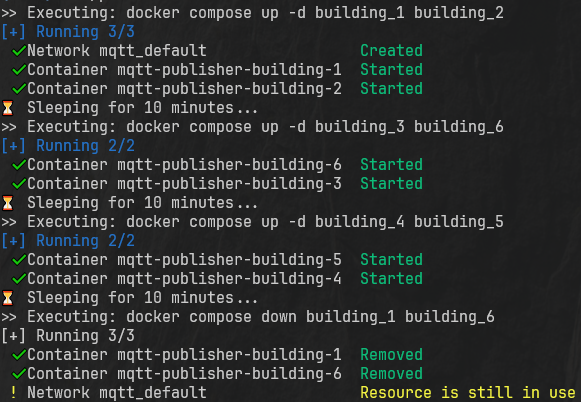
\includegraphics[width=\textwidth]{training-publish.png}
    \caption{Thực thi tệp mô phỏng gửi dữ liệu}
\end{figure}

\section{Hệ thống theo dõi, đánh giá, trực quan hóa dữ liệu}

\paragraph{Storm UI}

Triển khai Storm UI để cung cấp API cho phép Storm exporter thu thập các chỉ số.

\begin{figure}[H]
    \centering
    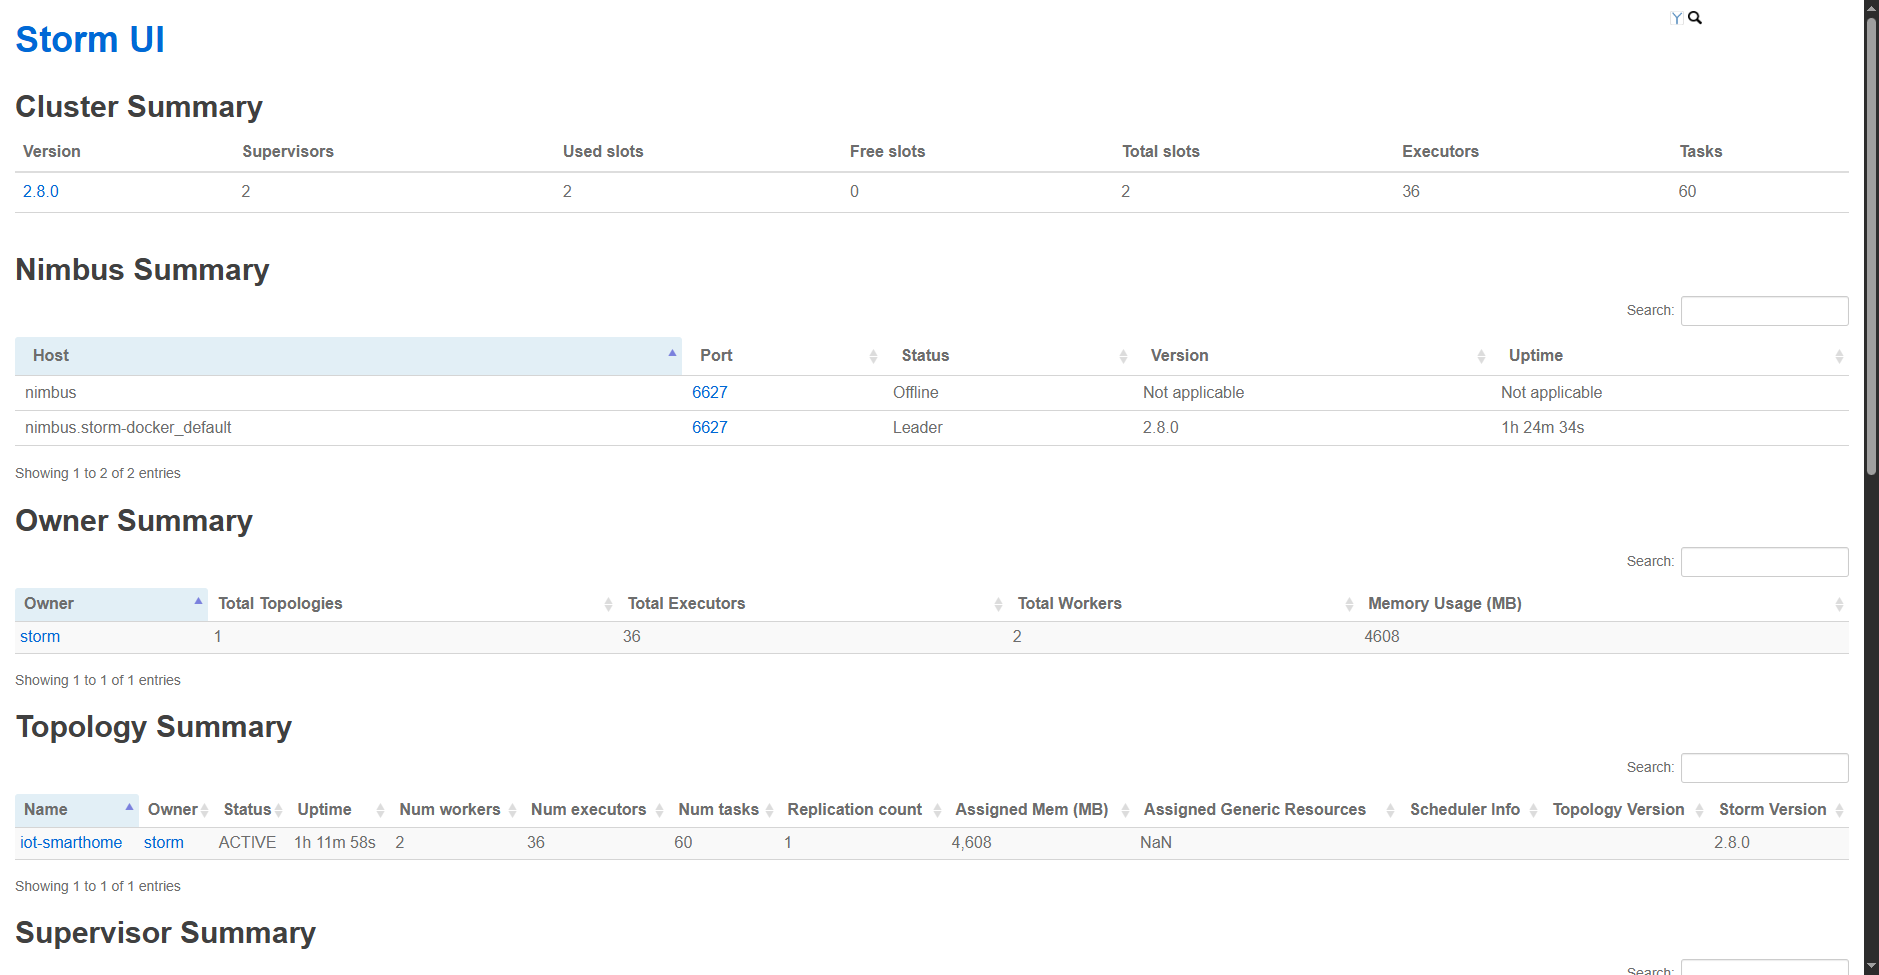
\includegraphics[width=\textwidth]{storm-ui.png}
    \caption{Storm UI}
\end{figure}

\begin{figure}
    \centering
    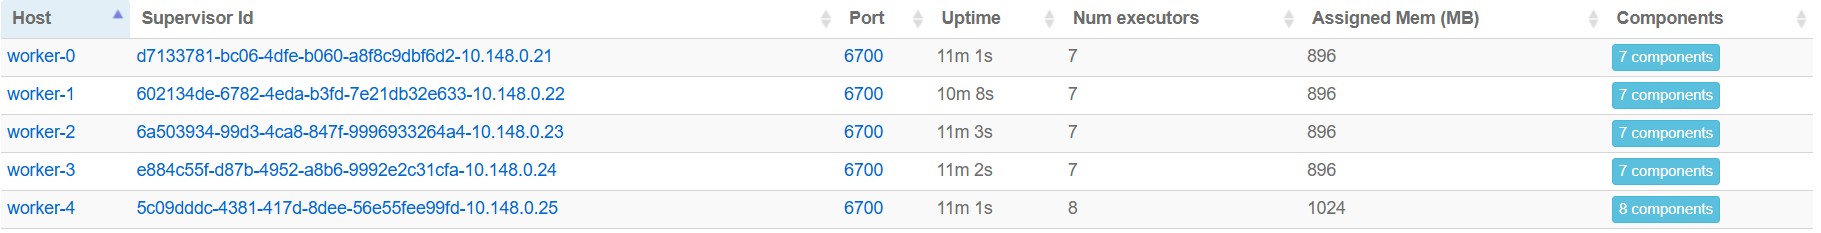
\includegraphics[width=\textwidth]{storm-ui-worker-resources.png}
    \caption{Theo dõi phân bố tài nguyên của các worker trên các supervisor}
\end{figure}

\paragraph{Storm Exporter}

Triển khai Storm exporter trên cùng tệp docker compose với storm-ui để thu thập các chỉ số từ topology và supervisor, sử dụng kèm với image socket-proxy \autocite{linuxserver_socket-proxy} để expose Docker socket làm phương tiện giúp Storm exporter đọc dữ liệu trong môi trường huấn luyện thông qua Docker API. Chương trình sử dụng các biến môi trường
\begin{itemize}
    \item STORM\_UI\_HOST: địa chỉ của chương trình Storm UI.
    \item REFRESH\_INTERVAL: khoảng thời gian giữa hai lần cập nhật chỉ số.
    \item EXPORTER\_LISTEN\_ADDR: địa chỉ storm exporter chạy.
    \item DOCKER\_HOST: địa chỉ để truy vấn Docker API.
\end{itemize}

\begin{lstlisting}[language=yaml, caption={Cấu hình triển khai Storm exporter}]
services:
  socket-proxy:
    image: lscr.io/linuxserver/socket-proxy:latest
    container_name: socket-proxy
    environment:
      - CONTAINERS=1
      - EVENTS=1
      - PING=1
      - VERSION=1
    volumes: [/var/run/docker.sock:/var/run/docker.sock:ro]
    restart: unless-stopped
    read_only: true
    tmpfs: [/run]

  storm-exporter:
    build:
      context: .
    container_name: storm-exporter
    restart: always
    environment:
      - STORM_UI_HOST=storm-ui:8081
      - REFRESH_INTERVAL=5
      - EXPORTER_LISTEN_ADDR=:8082
      - DOCKER_HOST=tcp://socket-proxy:2375
    ports: [8082:8082]
    depends_on: [socket-proxy]
\end{lstlisting}

\paragraph{Grafana}
Grafana được triển khai trên máy chủ nội bộ trong cả hai giai đoạn.

\begin{center}
    \begin{figure}[H]
        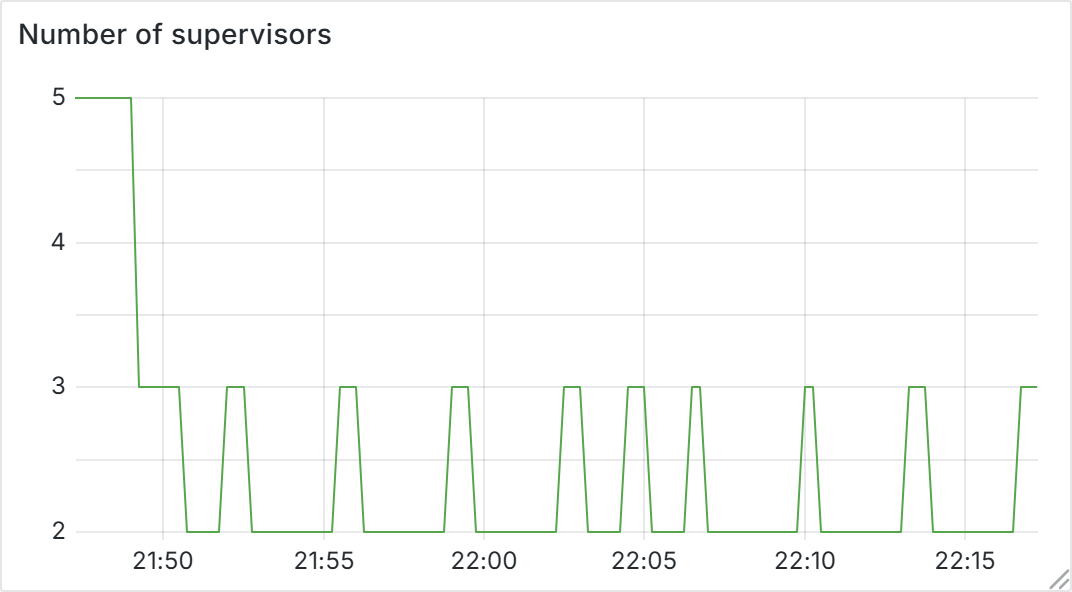
\includegraphics[width=\textwidth]{grafana-number-of-supervisor.png}
        \caption{Theo dõi số lượng supervisor theo thời gian của cụm Apache Storm}
    \end{figure}

    \begin{figure}[H]
        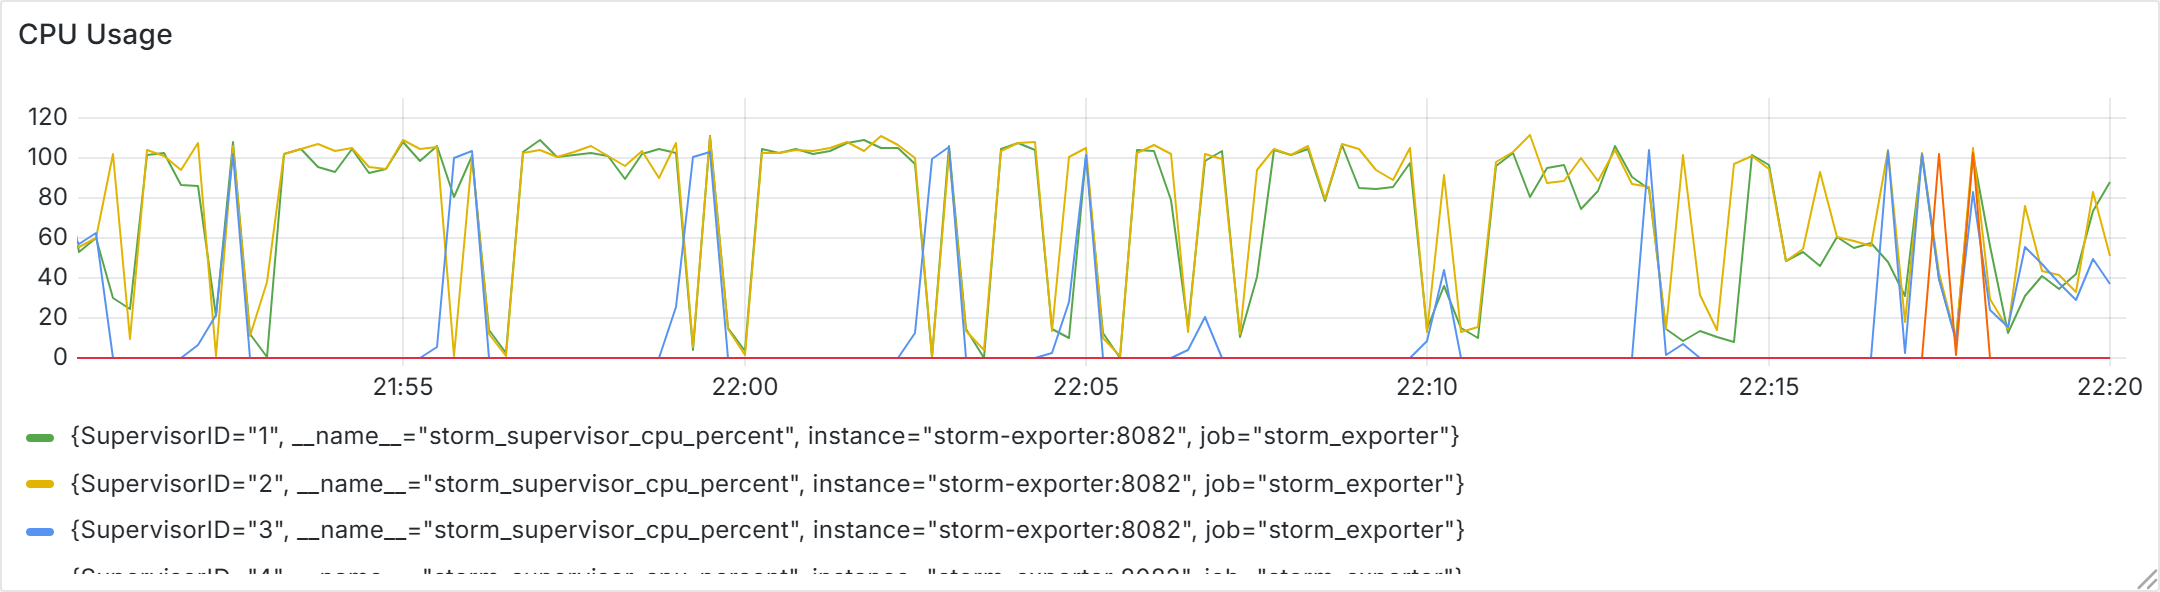
\includegraphics[width=\textwidth]{grafana-cpu-usage.png}
        \caption{Theo dõi tỷ lệ sử dụng \gls{cpu} của từng supervisor}
    \end{figure}
\end{center}

\section{Triển khai hệ thống dự đoán tài nguyên và co/dãn}

\subsection{Triển khai chương trình co/dãn tài nguyên}

Chương trình co/dãn tài nguyên được tác giả viết và lưu trữ trong thư mục autoscaler tại bộ mã nguồn của đồ án \autocite{lemionday_thesis_storm}. Để khởi chạy chương trình, có hai phương pháp:

\begin{itemize}
    \item Build và chạy chương trình tại cùng máy chủ với Storm nimbus. Khả dụng cho cả giai đoạn huấn luyện lẫn đánh giá. Lệnh chạy:
          \begin{verbatim}
go build -o build/storm-autoscaler
ENVIRONMENT=... build/storm-autoscaler
    \end{verbatim}
    \item Chạy chương trình thông qua image được đóng gói bởi Dockerfile cùng thư mục. Chỉ khả dụng trong giai đoạn đánh giá do không cần tương tác với Docker Compose. Lệnh chạy:
          \begin{verbatim}
docker build --tag storm-autoscaler:v1.0.0 .
docker run -d -e  ENVIRONMENT=... storm-autoscaler:v1.0.0
    \end{verbatim}
\end{itemize}
trong đó, các biến môi trường của chương trình
\begin{itemize}
    \item ENVIRONMENT: (\gls{gcp}/Docker) tương ứng với hai môi trường thử nghiệm (Docker) và đánh giá (\gls{gcp})
    \item PORT: cổng mà chương trình lắng nghe (mặc định 8083)
\end{itemize}

Sau khi triển khai, ta có thể đọc log của Storm autoscaler được hiển thị trên màn hình.

\begin{figure}[H]
    \centering
    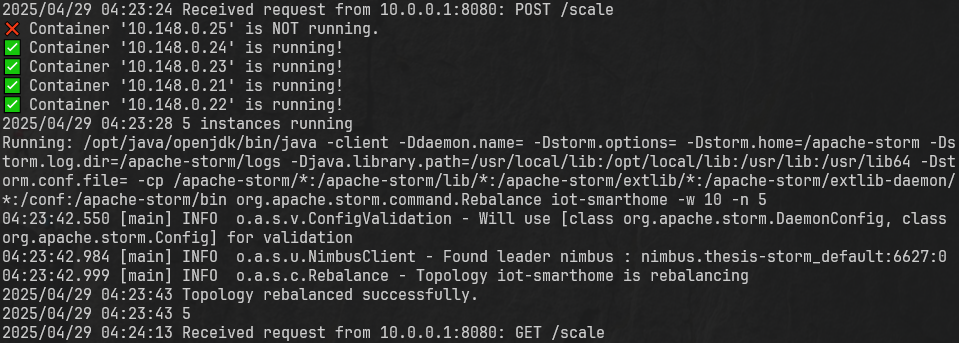
\includegraphics[width=\textwidth]{storm-autoscaler.png}
    \caption{Storm autoscaler}
\end{figure}

\subsection{Giai đoạn huấn luyện}

Giai đoạn này có tác dụng xây dựng và tối ưu hóa bảng mô hình cho thuật toán học tăng cường, để hệ thống có thể tiếp xúc, tạo cơ sở về các đánh giá đối với môi trường được mô phỏng, giúp tăng hiệu quả và tốc độ trong giai đoạn sau, giai đoạn đánh giá.

\subsubsection{Triển khai cụm Apache Storm}

Các dịch vụ Nimbus, UI, Zookeeper, Supervisor được chạy trên máy chủ local bằng mô phỏng kiến trúc Docker Compose. Trong đó Storm Supervisor được chạy theo chế độ nhân bản với số lượng tối đa là năm và số lượng tối thiểu là hai. Cấu hình của mỗi Supervisor là 550 MB RAM và 1 v\gls{cpu}.

\begin{lstlisting}[language=yaml, caption={Cấu hình của các supervisor}]
storm-supervisor:
    image: storm
    restart: always
    command: [storm, supervisor]
    volumes:
    - ./config/hosts:/etc/hosts:ro
    - ./config/storm.yml:/conf/storm.yaml
    deploy:
    replicas: 2
    resources:
        limits:
        memory: 550M
        cpus: 1
\end{lstlisting}

Do tất cả thành phần trên đều kết nối qua bridge network ảo của Docker được đảm bảo độ trễ giữa các dịch vụ không vượt quá 5ms - tương đương với độ trễ trong trung tâm dữ liệu. Mặc dù thành phần gửi dữ liệu (\gls{mqtt} publisher) và các thành phần của cụm Storm đều nằm trên máy chủ nội bộ, giữa chúng còn có thành phần liên kết là \gls{mqtt} broker được đặt tách biệt, vậy nên vẫn sẽ có độ trễ giống môi trường thật. Đây có thể coi như mô phỏng khá chính xác giữa môi trường trong giai đoạn huấn luyện với môi trường đánh giá hay thực tế sẽ được triển khai.

\subsubsection{Thao tác co/dãn tài nguyên}

Docker Compose cung cấp cơ chế chạy các dịch vụ dưới dạng nhân bản (replicas). Dịch vụ trong Docker Compose là một tập các container. Đây sẽ là cơ sở để điều chỉnh số lượng supervisor trong môi trường huấn luyện. Người dùng có thể dễ dàng điều chỉnh số lượng nhân bản của một dịch vụ - cụ thể ở đây là storm-supervisor thông qua lệnh sau:

\begin{verbatim}
docker compose up -d --scale storm-supervisor <number_of_replicas>
\end{verbatim}

Quá trình huấn luyện sẽ được triển khai như đã trình bày tại chương trước, mô hình được huấn luyện sẽ được liên tục cập nhật và lưu trữ tại ổ cứng theo các quy tắc đã định trước.

\subsection{Giai đoạn đánh giá}

Giai đoạn này thử nghiệm mô hình trên môi trường điện toán đám mây để kiểm tra hiệu năng thực tế, tính ổn định và khả năng thích ứng khi tải biến đổi.

\subsubsection{Triển khai máy ảo}

\begin{table}[h]
    \centering
    \resizebox{\textwidth}{!}{%
        \begin{tabular}{|l|l|l|l|l|l|l|}
            \hline
            Máy chủ           & Địa chỉ IP nội bộ    & \begin{tabular}[c]{@{}l@{}}Địa chỉ IP\\ công cộng\end{tabular} & Các dịch vụ chạy                                                                                                       & Cấu hình      & v\gls{cpu} & \begin{tabular}[c]{@{}l@{}}RAM\\ (GB)\end{tabular} \\ \hline
            storm-manager     & 10.148.0.20          & Có                                                             & \begin{tabular}[c]{@{}l@{}}Storm Nimbus\\ Storm UI\\ Zookeeper\\ MySQL\\ Prometheus\\ Wireguard\\ Ansible\end{tabular} & e2-standard-2 & 2          & 8                                                  \\ \hline
            worker{[}0...4{]} & 10.148.0.{[}21-25{]} & Không                                                          & \begin{tabular}[c]{@{}l@{}}Supervisor\\ Container exporter\end{tabular}                                                & e2-micro      & 2          & 1                                                  \\ \hline
            forecast          & Không                & Có                                                             & \begin{tabular}[c]{@{}l@{}}Storm forecast\\ Wireguard\end{tabular}                                                     & e2-micro      & 2          & 1                                                  \\ \hline
            publisher         & 10..148.0.11         & Không                                                          & \gls{mqtt} publisher                                                                                                   & e2-micro      & 2          & 1                                                  \\ \hline
        \end{tabular}%
    }
    \caption{Bảng phân bố các dịch vụ trên các máy chủ \gls{gcp}}
    \label{tab:gcp-services-distribution}
\end{table}

\begin{table}[h]
    \centering
    \resizebox{\textwidth}{!}{%
        \begin{tabular}{|l|l|l|l|l|}
            \hline
            Máy chủ        & Tên máy chủ   & Vị trí    & Vai trò trong Wireguard & Địa chỉ IP Wireguard \\ \hline
            Storm manager  & storm-manager & \gls{gcp} & Server                  & 10.0.0.1             \\ \hline
            Storm forecast & forecast      & \gls{gcp} & Peer01                  & 10.0.0.2             \\ \hline
            Máy chủ cục bộ & localhost     & Cục bộ    & Peer02                  & 10.0.0.3             \\ \hline
        \end{tabular}%
    }
    \caption{Phân bố vai trò và địa chỉ IP của các máy chủ trong VPN Wireguard}
    \label{tab:wireguard-distribution}
\end{table}

\begin{figure}[h]
    \centering
    \includegraphics[width=\textwidth]{deployment-gcp.drawio.png}
    \caption{Sơ đồ triển khai các máy ảo trên \gls{gcp}}
    \label{fig:deployment-gcp}
\end{figure}

\begin{figure}[h]
    \centering
    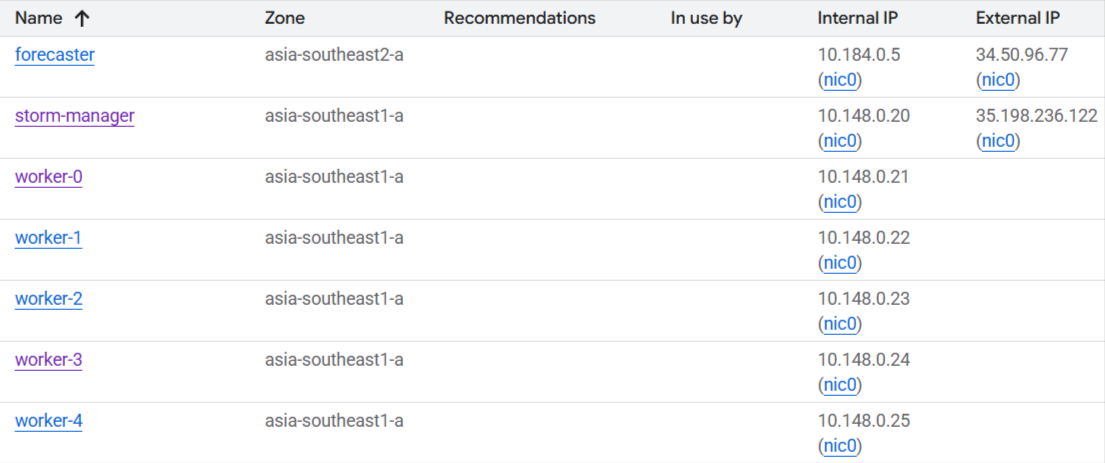
\includegraphics[width=\textwidth]{gcp-compute-engines.png}
    \caption{Khởi tạo máy ảo trên môi trường điện toán đám mây \gls{gcp}}
\end{figure}

% Please add the following required packages to your document preamble:
% \usepackage{graphicx}
\begin{table}[h]
    \centering
    \resizebox{\textwidth}{!}{%
        \begin{tabular}{|l|l|l|l|l|l|}
            \hline
            Tên              & Nguồn                 & Hướng dữ liệu & Giao thức & Cổng                                                                     & Đối tượng áp dụng                                                        \\ \hline
            allow-ssh        & 0.0.0.0/0             & Vào/ra        & tcp       & 22                                                                       & Tất cả                                                                   \\ \hline
            allow\_wireguard & 0.0.0.0/0             & Vào           & udp       & 51820                                                                    & Tất cả                                                                   \\ \hline
            storm\_firewall  & Dải IP nội bộ của VPC & Vào/ra        & tcp       & \begin{tabular}[c]{@{}l@{}}6627\\ 6628\\ 8000\\ 2181\\ 6700\end{tabular} & \begin{tabular}[c]{@{}l@{}}storm-manager\\ worker-{[}0-4{]}\end{tabular} \\ \hline
            allow\_mysql     & Dải IP nội bộ của VPC & Vào           & tcp       & 3306                                                                     & storm-manager                                                            \\ \hline
        \end{tabular}%
    }
    \caption{Bảng danh sách các quy tắc tường lửa}
    \label{tab:firewall-rules}
\end{table}

Danh sách các máy chủ cùng với địa chỉ IP, cấu hình và các dịch vụ chúng chạy được liệt kê trong bảng \ref{tab:gcp-services-distribution}, sơ đồ thiết kế triển khai được minh họa trong hình \ref{fig:deployment-gcp}. Nhằm nâng cao tính bảo mật đồng thời đơn giản hóa việc áp dụng các quy tắc tường lửa, tác giả đã triển khai thêm hệ thống VPN WireGuard cho Storm manager, Storm forecast cùng với máy chủ cục bộ, cấu hình chi tiết được liệt kê trong bảng \ref{tab:wireguard-distribution}. Đối với các máy ảo trong cùng một VPC của \gls{gcp}, cụ thể là Storm manager và các worker, việc triển khai WireGuard là không cần thiết do đã có hệ thống tường lửa có sẵn của \gls{gcp} đồng thời các worker truy cập internet thông qua NAT router của \gls{gcp} nên khả năng bị tấn công sẽ không có, do vậy ta chỉ cần mở các cổng tường lửa tương ứng với các cổng dịch vụ và thiết lập nguồn gửi trong cùng VPC là có thể đảm bảo hệ thống sẽ hoạt động chính xác. Danh sách các quy tắc tường lửa hệ thống áp dụng đã được liệt kê trong bảng \ref{tab:firewall-rules}.

Quá trình triển khai các máy ảo trên nền tảng \gls{gcp} được tự động hóa thông qua công cụ Terraform, cho phép khởi tạo đồng thời nhiều máy ảo worker chạy Storm supervisor, dễ dàng điều chỉnh cấu hình và số lượng các worker. Mã nguồn quản lý toàn bộ kiến trúc hạ tầng của đồ án cùng với đó là các script khởi chạy dịch vụ được tác giả viết và lưu trữ trong thư mục cloud của bộ mã nguồn của đồ án \autocite{lemionday_thesis_storm}.

Trong phạm vi luận án này, tác giả đã sử dụng 5 máy ảo worker. Các dịch vụ Storm supervisor được đóng gói và vận hành trong các container trên các máy ảo này, tạo điều kiện thuận lợi cho việc co/dãn dịch vụ supervisor một cách linh hoạt. Về mặt chi phí, mô hình dự đoán tài nguyên cho phép tác giả cân nhắc việc sử dụng các máy ảo Spot VMs cho một số lượng worker nhất định, tận dụng dung lượng dư thừa của trung tâm dữ liệu trong thời gian thấp điểm để giảm chi phí vận hành máy ảo đến 91\% theo chính sách tính giá của \acrshort{gcp}. Mặt khác, việc đặt chỗ trước (reserved instances) một số lượng máy ảo cũng là một giải pháp tiềm năng để tối ưu hóa chi phí, khi tài nguyên nhàn rỗi trong giai đoạn thấp điểm có thể được sử dụng cho các tác vụ tính toán khác, thay vì chỉ dành riêng cho hệ thống xử lý dữ liệu của ứng dụng SmartHome. Việc kết hợp các chiến lược này có tiềm năng giảm đáng kể tổng chi phí hệ thống.

\newpage

\begin{lstlisting}[language=HCL, caption={Cấu hình khởi tạo máy ảo worker chạy Storm supervisor}]
resource "google_compute_instance" "worker" {
    count        = 5
    name         = "worker-${count.index}"
    machine_type = var.worker_machine_type
    zone         = var.zone

    boot_disk {
        initialize_params {
        image = "debian-cloud/debian-11"
        }
    }

    network_interface {
        network    = google_compute_network.storm_network.name
        network_ip = var.worker_internal_ips[count.index]
    }

    metadata_startup_script = join("\n",
        [
        file("./scripts/setup_docker.sh"),
        file("./scripts/setup_storm.sh"),
        file("./scripts/setup_storm_supervisor.sh"),
        file("./scripts/setup_docker_exporter.sh")
        ]
    )

    metadata = {
        ssh-keys = "storm:${file("./secrets/storm.pub")}"
    }

    tags = ["storm", "wireguard", "docker-access"]
}
\end{lstlisting}

\paragraph{Cấu hình Nimbus}

Do nền tảng Apache Storm không được thiết kế phù hợp đối với hệ thống co/dãn tài nguyên các supervisor, nguyên nhân là do cơ chế danh sách đen. Trong khoảng thời gian dài nếu nimbus không nhận được phản hồi từ các supervisor, chúng sẽ bị đưa vào danh sách đen và phải sau một khoảng thời gian nhất định thì các supervisor này mới có thể được loại bỏ khỏi danh sách đen.

Các supervisor ở trong danh sách đen sẽ không được phân phối công việc bởi nimbus, điều này ảnh hưởng rất lớn đến hoạt động của hệ thống khi chúng gây ra hai vấn đề. Vấn đề thứ nhất, số lượng các supervisor được phân phối công việc với số lượng supervisor trong tái cấu trúc (rebalance) không khớp nhau từ đó gây ra thiếu slot cần thiết để thực thi topology, thậm chí có thể khiến hệ thống ngừng xử lý dữ liệu. Vấn đề còn lại, do không được phân phối công việc, supervisor sẽ không có ý nghĩa trong topology, gây lãng phí tài nguyên.

Vì lý do này thời gian để các supervisor được loại bỏ khỏi danh sách đen phải đủ ngắn để không bị đưa vào danh sách đen khi được bật trở lại sau khi tắt. Tại đây blacklist được cấu hình chu kỳ dài 30 giây kể từ khi supervisor bị đưa vào danh sách đen đến khi được loại bỏ, tương ứng với thời gian chờ giữa các lần co/dãn.

\begin{lstlisting}[language=yaml, caption={Cấu hình Nimbus node}]
storm.zookeeper.servers: [zookeeper]
nimbus.seeds: [nimbus]
ui.port: 8081

supervisor.slots.ports: [6700]

storm.blacklist.scheduler.tolerance.time.secs: 30
blacklist.scheduler.tolerance.time.secs: 30
blacklist.scheduler.tolerance.count: 1
blacklist.scheduler.resume.time.secs: 30

storm.local.hostname: "nimbus.thesis-storm_default"
\end{lstlisting}

\paragraph{Triển khai ứng dụng xử lý dữ liệu SmartHome lên cụm Apache Storm}

Mã nguồn của topology sử dụng mã nguồn chương trình xử lý dữ liệu nhà thông minh xây dựng trên nền tảng Apache Storm \autocite{fimocodestormsmarthome} với một thay đổi nhỏ là \gls{mqtt} broker được đổi thành broker.emqx.io. Đầu tiên ta tiến hành đẩy topology đã được biên dịch trên máy chủ cục bộ lên máy ảo storm-manager.

\begin{verbatim}
gcloud compute scp \\
./stormsmarthome/target/Storm-IOTdata-1.0-SNAPSHOT-jar-with-dependencies.jar \\
storm@storm-manager:~/thesis-storm/stormsmarthome/target   
\end{verbatim}

Sau đó tiến hành triển khai topology tại container nimbus.

\begin{verbatim}
docker exec nimbus storm jar \\
    /topologies/Storm-IOTdata-1.0-SNAPSHOT-jar-with-dependencies.jar \\
    com.storm.iotdata.MainTopo
\end{verbatim}

\begin{figure}
    \centering
    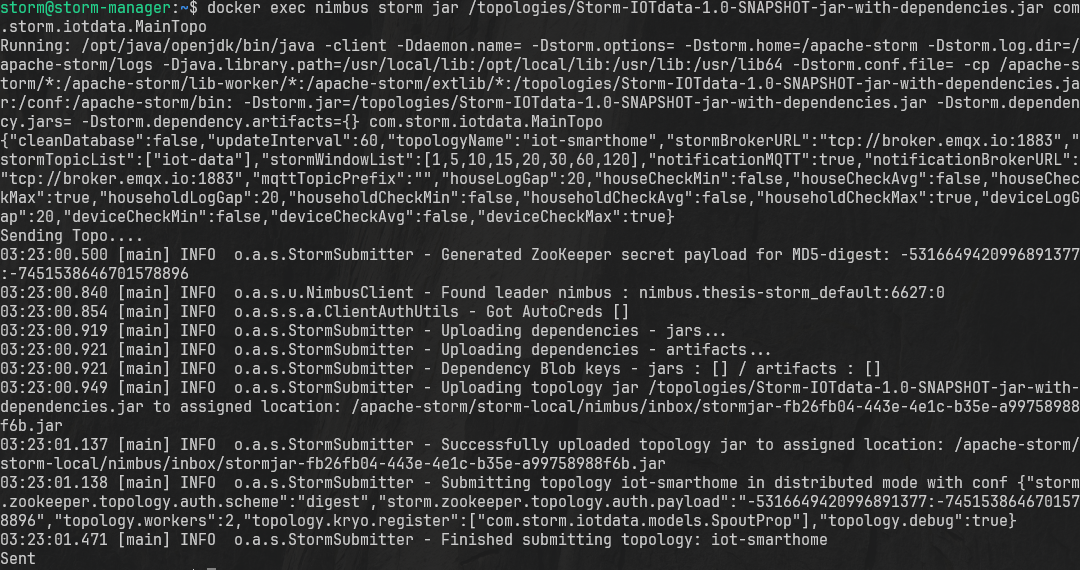
\includegraphics[width=\textwidth]{deploy-topology.png}
    \caption{Triển khai topology lên Apache Storm}
\end{figure}

\paragraph{Máy ảo supervisor}

Trên mỗi máy ảo supervisor sẽ triển khai hai dịch vụ chính: Container exporter \autocite{shayan_ghani_container_exporter} và Storm supervisor. Trong đó, Container exporter đảm nhiệm việc cung cấp các thông số giám sát hệ thống thông qua đường dẫn \textit{/metrics}, mặc định được lắng nghe tại cổng \textit{8000}. Khác với giai đoạn huấn luyện, khi Storm exporter trực tiếp thu thập dữ liệu từ Docker API của các supervisor cục bộ, trong môi trường triển khai thực tế, nó sẽ thu thập dữ liệu từ đường dẫn \textit{/metrics} của các máy ảo worker. Sau đó, Storm exporter tổng hợp, chuyển đổi tên các metric và bổ sung nhãn để đảm bảo tính thống nhất giữa các môi trường với các truy vấn dữ liệu của hệ thống Storm forecast.

\begin{lstlisting}[language=yaml, caption={Cấu hình các dịch vụ chạy trên máy ảo supervisor}]
services:
    cxp:
        image: devopsteen/cxp:latest
        container_name: container-exporter
        volumes: [/var/run/docker.sock:/var/run/docker.sock]
        ports: [8000:8000]
        restart: always

    storm-supervisor:
        image: storm
        restart: always
        command: [storm, supervisor]
        network_mode: host
        volumes:
        - ./config/hosts.cloud:/etc/hosts:ro
        - ./config/storm.cloud.yml:/conf/storm.yaml
        deploy:
        resources:
            limits:
            memory: 550M
            cpus: 1
\end{lstlisting}

Mỗi supervisor chỉ sử dụng một port duy nhất cho chúng chỉ được cấp 1 \gls{cpu}, giới hạn bộ nhớ và \gls{cpu} lần lượt là 550Mb và 100 - tương ứng với 1 \gls{cpu}.
\begin{lstlisting}[language=yaml, caption={Cấu hình của dịch vụ supervisor}]
storm.zookeeper.servers: [10.148.0.20]
nimbus.seeds: [nimbus.thesis-storm_default]

supervisor.slots.ports:
- 6700

supervisor.memory.capacity.mb: 550
supervisor.cpu.capacity: 100
\end{lstlisting}

\subsection{Triển khai chương trình co/dãn - Storm forecast}

Mã nguồn chương trình được tác giả đồ án viết và lưu tại thư mục forecast trong bộ mã nguồn của đồ án \autocite{lemionday_thesis_storm}. Hai chương trình chạy tương ứng với hai mô hình học tăng cường.

\begin{itemize}
    \item \textbf{Học tăng cường Q}:
          \begin{verbatim}
python3 -m q_learning.agent
    \end{verbatim}
    \item \textbf{Học tăng cường Q sâu}:
          \begin{verbatim}
python3 -m dq_learning.agent
    \end{verbatim}
\end{itemize}

trong đó các biến môi trường
\begin{itemize}
    \item PROMETHEUS\_URL (mặc định: localhost:9090): Đường dẫn đến Prometheus.
    \item AUTOSCALER\_URL (mặc định: localhost:8083): Đường dẫn đến chương trình Autoscaler.
\end{itemize}

Sau khi bắt đầu khởi chạy chương trình, nếu có thể tìm thấy tệp mô hình đã được lưu qscale.npy (Học tăng cường Q) và dqscale.pt (Học tăng cường Q sâu), chúng sẽ được tải để sử dụng.

\begin{figure}[H]
    \centering
    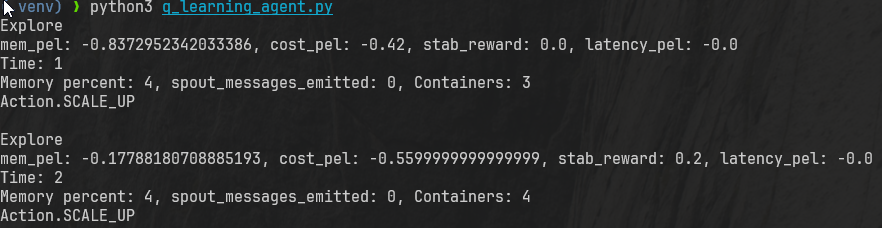
\includegraphics[width=\textwidth]{training-start.png}
    \caption{Bắt đầu quá trình huấn luyện học tăng cường Q}
    \label{fig:training-start}
\end{figure}

\begin{figure}[H]
    \centering
    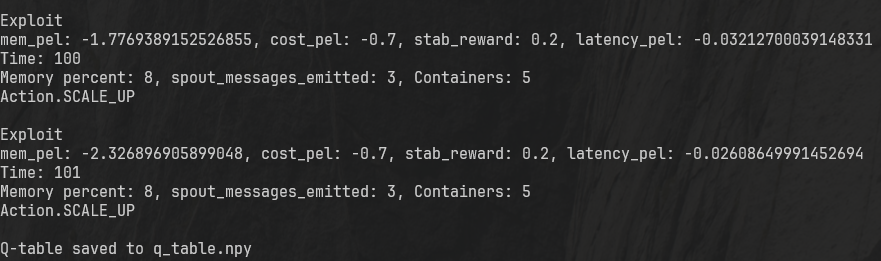
\includegraphics[width=\textwidth]{training-save-q-table.png}
    \caption{Lưu bảng giá trị Q sau khi huấn luyện}
    \label{fig:training-save}
\end{figure}

\begin{figure}[H]
    \centering
    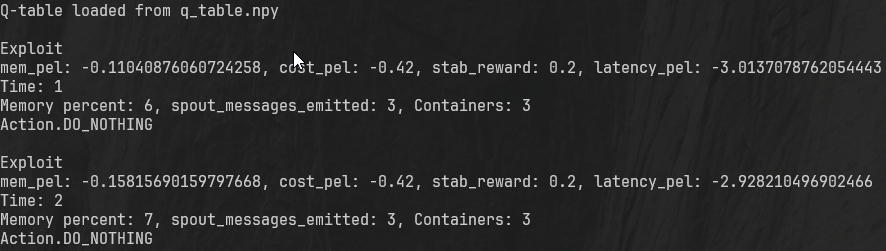
\includegraphics[width=\textwidth]{evaluation-01-start.png}
    \caption{Sử dụng bảng giá trị Q đã lưu để tiến hành đánh giá}
    \label{fig:evaluate-start}
\end{figure}

\begin{figure}[H]
    \centering
    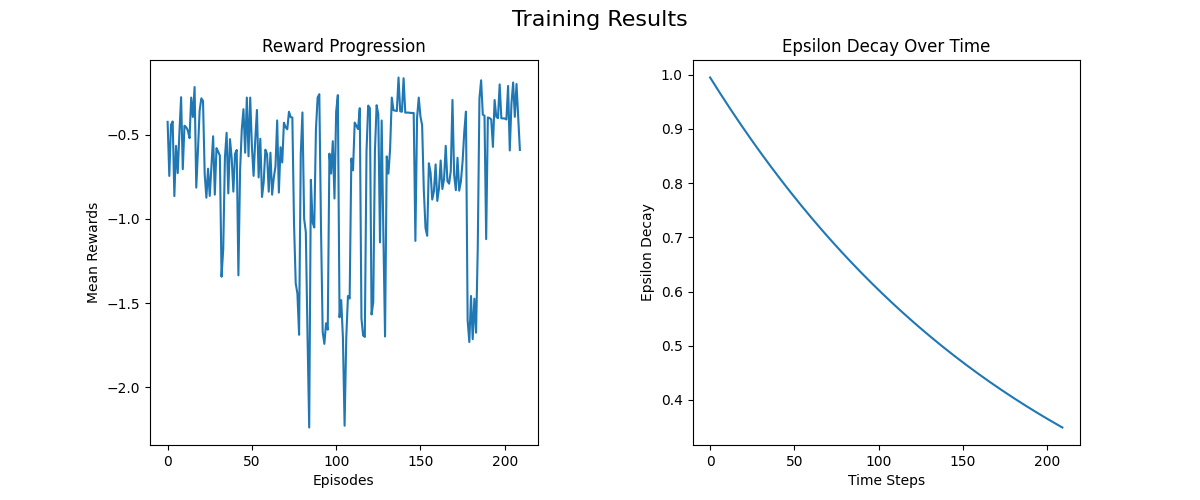
\includegraphics[width=\textwidth]{qscale-training-results.png}
    \caption{Đồ thị biểu diễn phần thưởng của mỗi hành động và các giá trị của epsilon sau mỗi lần thực hiện hành động}
    \label{fig:result-graph}
\end{figure}

Đồ thị được biểu diễn tại hình \ref{fig:result-graph} biểu diễn phần thưởng được tính toán từ trạng thái kế tiếp sau mỗi hành động của tác nhân và giá trị $\epsilon$ giảm dần theo thời gian tương ứng với hiểu biết của tác nhân về môi trường tăng lên theo thời gian và tỷ lệ khám phá giảm dần.